%\vspace{-0.475cm}
\section{Medial Fragments: Superpixels  and Contours won't do}
\label{sec:atomic:fragments}
%\vspace{-0.28cm}
Two types of representations suggest themselves on which various grouping
operations can operate:\ \textit{superpixels} and \textit{contour fragments}. It is argued
below that neither is sufficient for the purpose of building multiple hypotheses
in the face of realistic levels of ambiguity and clutter~\cite{Tamrakar:Kimia:POCV04}.  Instead we motivate and adopt \textit{medial fragments}~\cite{Tamrakar:Kimia:POCV04}. 


\textbf{Superpixels} are the basic unit of reasoning about object fragments resulting
from grouping pixels into region fragments based on regional 
homogeneity~\cite{Ren:Malik:ICCV03,Ahuja:Todorovic:CVPR08,malisiewicz:bmvc07}, \etc\  One
main difficulty with the boundaries of  superpixels is that it is not clear
which portions are meaningful boundaries and which are simply delimiters of the grouped pixels. These latter contours are more a product of the dynamics
of the grouping process than an indicator of underlying structure, \eg,
the pink-yellow boundary in Figure~\ref{figure:combinatorial:possibilities}b. The ambiguity created by the presence
of these artifactual boundaries among meaningful boundaries limits the use of  grouping based on contours.
% \begin{figure}[!h]
% \centerline{
% {\footnotesize\textit{a}}
% 
\includegraphics[height=0.22\linewidth]{figs/shaded-torus.png}
% {\footnotesize\textit{b}}
% 
\includegraphics[height=0.22\linewidth]{figs/shaded-torus-segmentation.png}
% {\footnotesize\textit{c}}
% \includegraphics[height=0.22\linewidth]{figs/koenderink-contour-end-1.png}
% {\footnotesize\textit{d}}
% 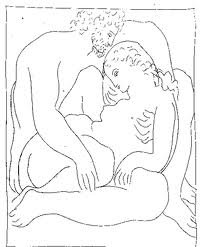
\includegraphics[height=0.22\linewidth]{figs/picasso-hands.png}
% %\includegraphics[height=0.2\linewidth]{figs/Prometheus-Brennan.png}
% %\hspace{-0.1cm}\includegraphics[height=0.2\linewidth]{figs/Prometheus-Brennan-k_12.pdf}
% }
%   \caption{\FigureFont
%   \label{fig:region:issues}
%   (a,b) Region-based grouping produce ``superpixels'' with boundaries composed
%   of both meaningful contours as well as artifactual boundaries resulting
%   from the dynamics of the grouping process which delimits adjacent regions
%   but does not lay claim to boundary-hood. Superpixels cannot represent
% contours that end, (c) from \cite{Koenderink:VanDoorn:Perception82} and
% (d) a Picasso drawing.   }
% %\vspace{-0.35cm}
%\end{figure}

\begin{figure}[!h]
%\vspace{-0.5cm}
\centering
 % {\footnotesize\textit{(a)}} \includegraphics[width=0.1225\linewidth]{figs/place_holder.pdf}
{\footnotesize\textit{a}}

\includegraphics[width=0.28\linewidth]{figs/shaded-torus.jpg}
{\footnotesize\textit{b}} 
\includegraphics[width=0.28\linewidth]{figs/shaded-torus-segmentation.jpg}
{\footnotesize\textit{c}} 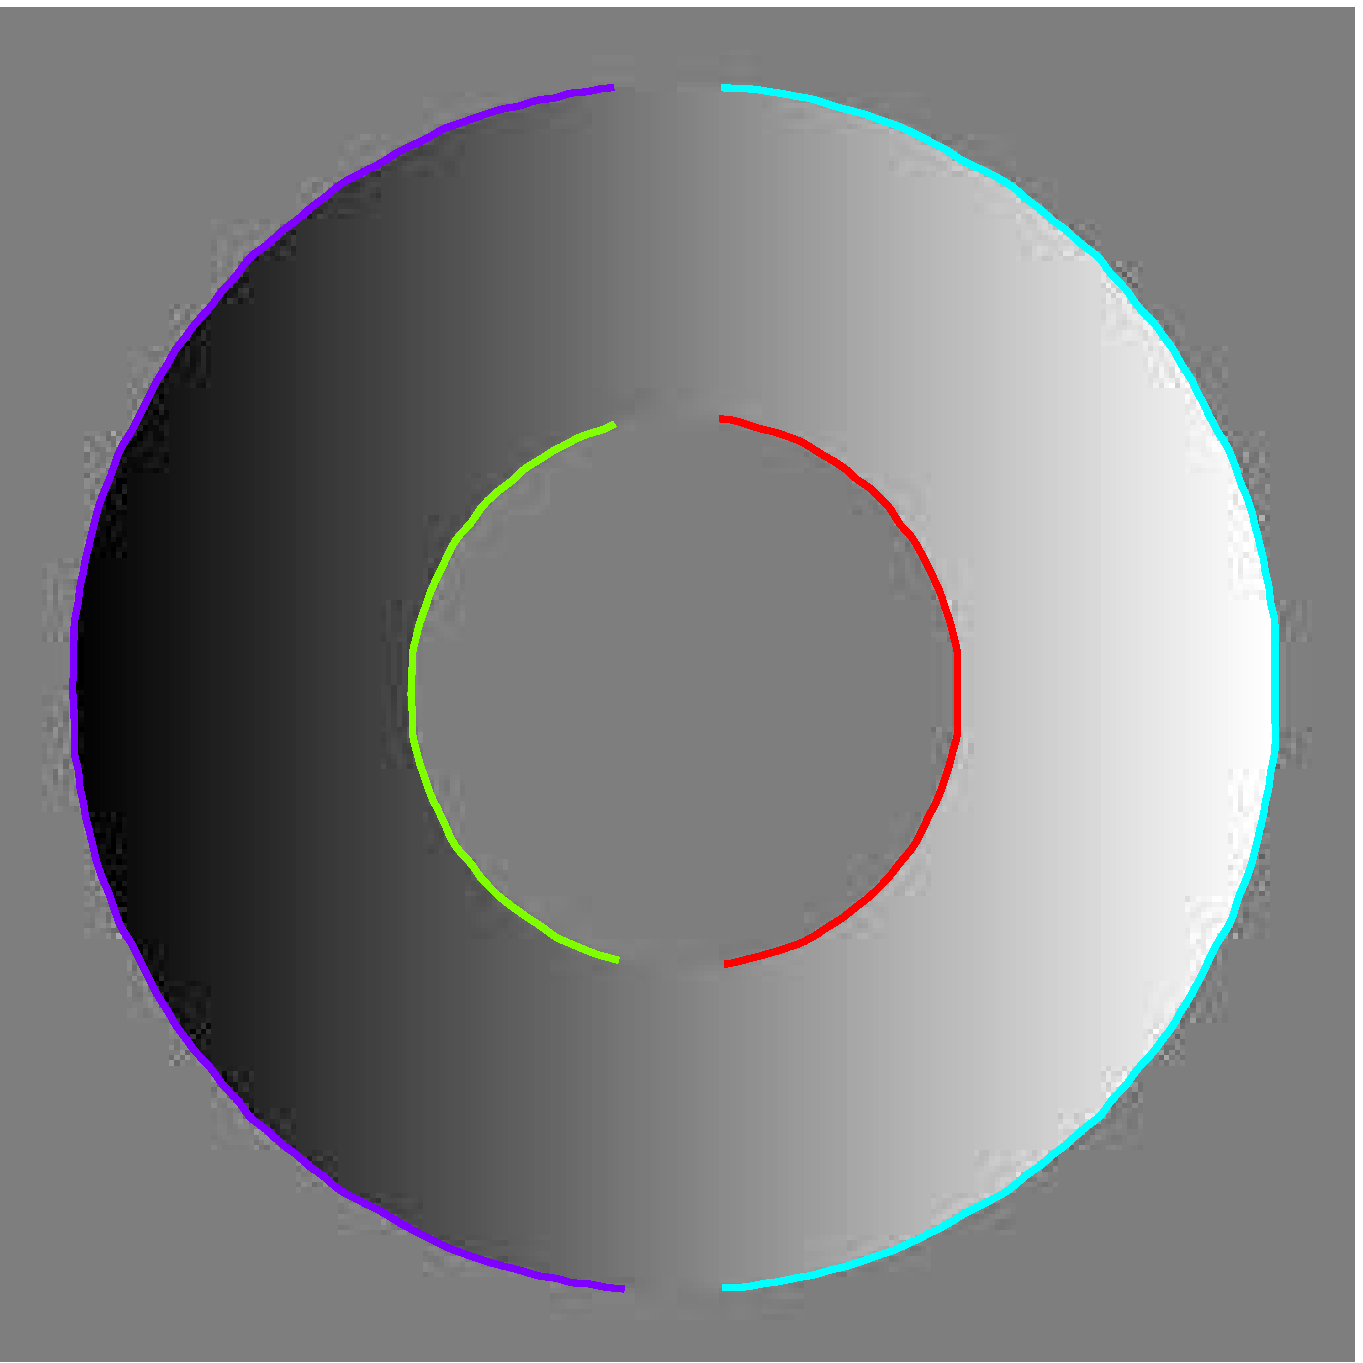
\includegraphics[width=0.28\linewidth]{figs/torus_contours_multi_color.pdf}
\\
%{\footnotesize\textit{(d)}}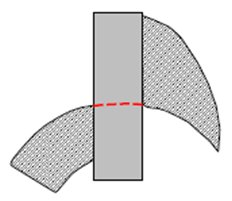
\includegraphics[width=0.1225\linewidth]{figs/contour-but-not-region.png}
%{\footnotesize\textit{(e)}} \includegraphics[width=0.1225\linewidth]{figs/competition-between-two-regions.png}
{\footnotesize\textit{d}} 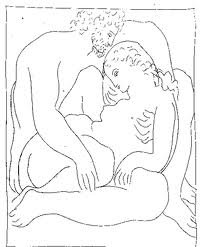
\includegraphics[height=0.15\textwidth]{figs/picasso-hands.jpg}
\vbox{
\hbox{
{\footnotesize\textit{e}}
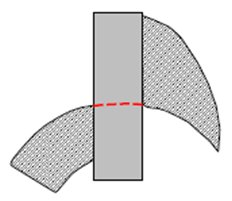
\includegraphics[height=0.15\linewidth]{figs/contour-but-not-region.jpg}
%\includegraphics[height=0.08\linewidth]{figs/figural-continuity-1.png}
{\footnotesize\textit{f}}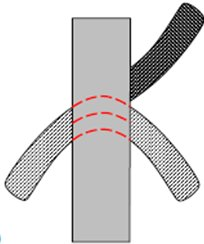
\includegraphics[height=0.15\linewidth]{figs/figural-continuity-2.jpg}
%{\footnotesize\textit{f}}\includegraphics[height=0.06\linewidth]{figs/good-continuation-1.png}
}
\hbox{
{\footnotesize\textit{g)}}
\includegraphics[height=0.1\linewidth]{figs/good-continuation-3.jpg}
%{\footnotesize\textit{h\includegraphics[height=0.056\linewidth]{figs/good-continuation-2.png}}}
{\footnotesize\textit{h}}
\includegraphics[height=0.1\linewidth]{figs/good-continuation-4.jpg}
}
}
% \hbox[2cm]{\includegraphics{figs/one-contour-between-two-others.png}
% \includegraphics{figs/one-contour-supports-another.png}
% \includegraphics{figs/one-gap-supports-another.png}}
{\footnotesize\textit{i}}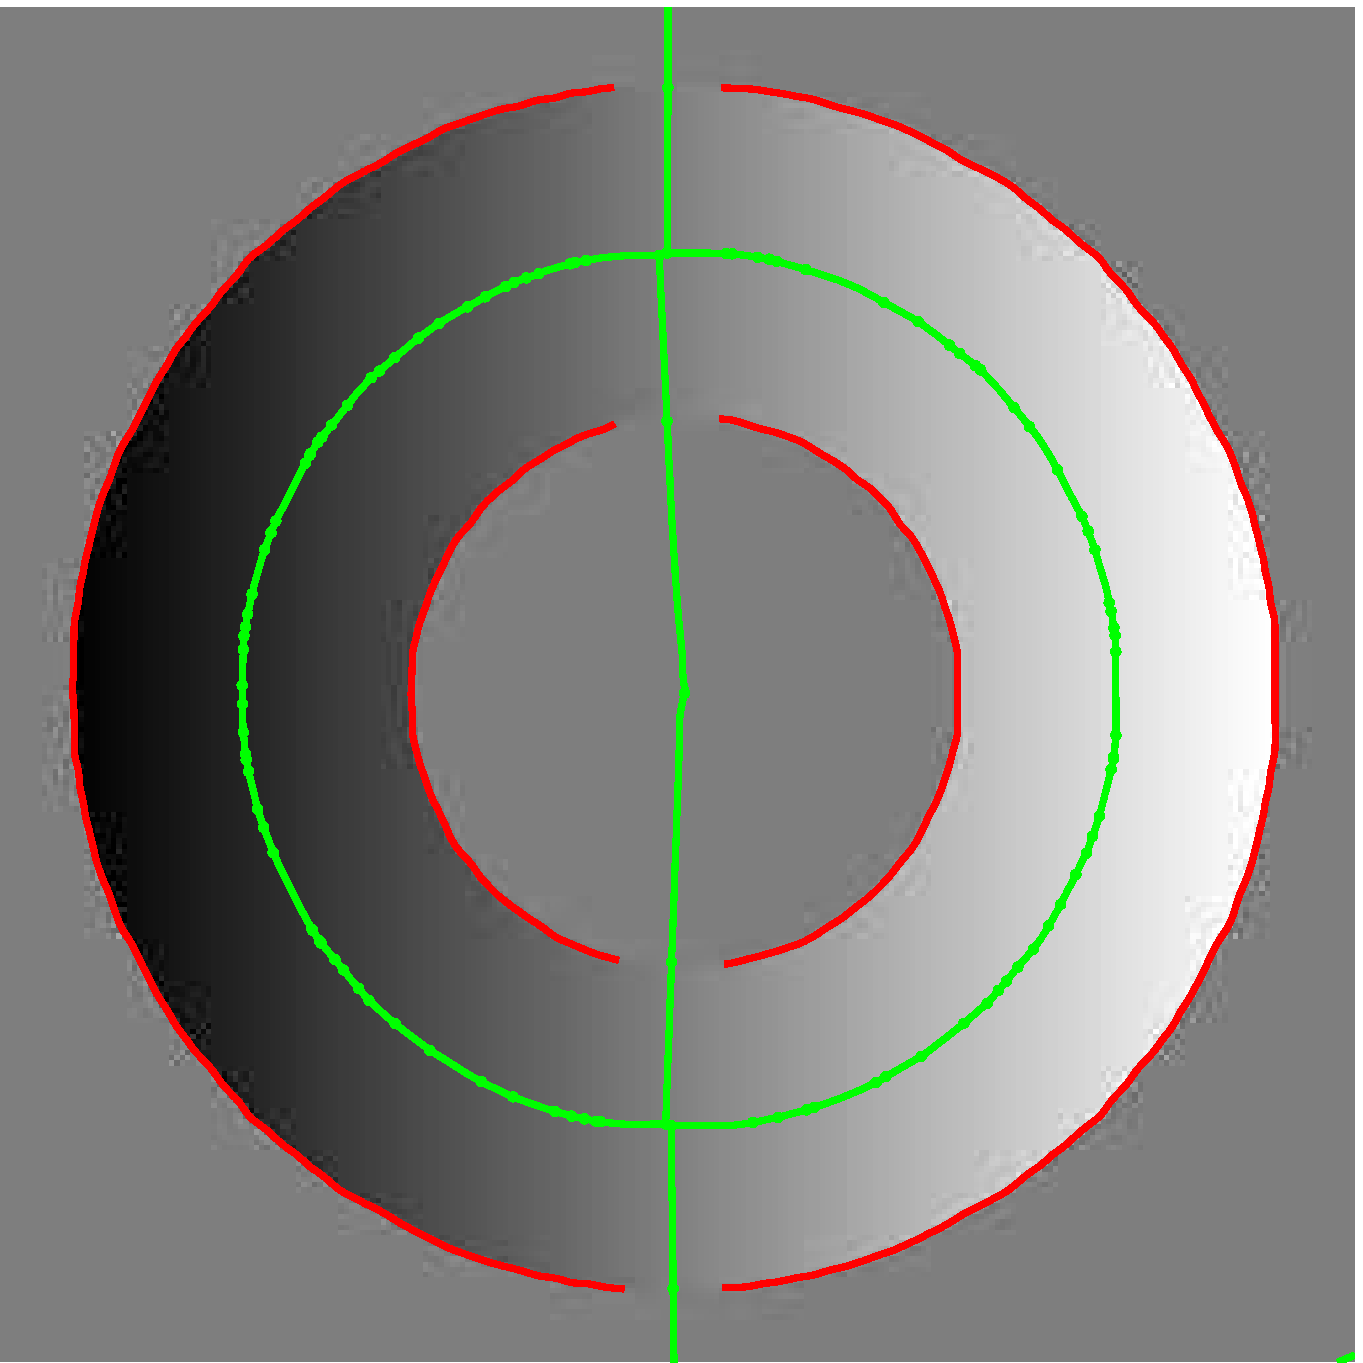
\includegraphics[width=0.23\linewidth]{figs/torus_contours_shocks.pdf}
%\textit{k} \hspace{-0.0512cm}
%  \includegraphics[width=0.135\linewidth]{figs/place_holder.pdf}
%\vspace{-0.2cm}
  \caption{\FigureFont (a,b) The use of superpixels is not appropriate in our
approach because (i) artifactual boundaries (say the contour between pink
and yellow regions) are not differentiated from actual boundaries,   and
(ii) the representation does not identify gap endpoints,  required to identify completion candidates. (c) contour fragment endpoints identify potential gaps. (d) many image contours are not closed (e-f)
appearance continuity is a powerful cue in grouping. The spatial interaction
among contours prevents some gaps from being considered (g), while supporting
others\ (h). (i) The shock graph pairs image contours. }
 \label{figure:combinatorial:possibilities}
%\vspace{-0.751cm}
 \end{figure}

Another fundamental difficulty in region-based representation is the inability to represent contours that end, Figure~\ref{figure:combinatorial:possibilities}d, which among others,  significantly limits the detection of gaps,
\eg, as present in the bottom and top portions of the inner and outer circles
in the shaded torus of Figure~\ref{figure:combinatorial:possibilities}a; It is difficult to work with gaps in the superpixel representation, Figure~\ref{figure:combinatorial:possibilities}b, because end-points of contours are
not represented.



  
% \begin{figure}[!h]
% {\footnotesize\textit{a}}
% \includegraphics[height=0.076\linewidth]{figs/good-continuation-1.png}
% {\footnotesize\textit{b}}
% \includegraphics[height=0.076\linewidth]{figs/good-continuation-2.png}
% {\footnotesize\textit{c}}
% 
\includegraphics[height=0.076\linewidth]{figs/good-continuation-3.png}
% {\footnotesize\textit{d}}
% 
\includegraphics[height=0.076\linewidth]{figs/good-continuation-4.png}
% {\footnotesize\textit{e}}
% \includegraphics[height=0.076\linewidth]{figs/good-continuation-5.png}
% {\footnotesize\textit{f}}
% \includegraphics[height=0.076\linewidth]{figs/appearance-continuity-1.png}
% {\footnotesize\textit{g}}
% \includegraphics[height=0.076\linewidth]{figs/appearance-continuity-2.png}
%   \caption{\FigureFont
%   \label{fig:contour:continuity}
%   The Gestalt notion of good continuation disambiguates between  the two situations in (a,b), but cannot detect interaction from related contours
% (c-e), which require a notion of figural continuity. (f,g) Appearance continuity is another significant cue. 
%   }
% \end{figure}

\textbf{Curve fragments} are often viewed as a precursor to figure-ground segregation and for formulating the Gestalt notion of good continuation,
Figure~\ref{figure:combinatorial:possibilities}c,
\eg, using elastica \cite{Mumford:Elastic:1994,Williams:Jacobs:NC95} or using the Euler Spiral \cite{Kimia:Euler:Spiral:IJCV03}. Good continuation is used to disambiguate grouping choices. However, a contour representation cannot take into account the interaction of nearby contours  which may invalidate a completion,
Figure~\ref{figure:combinatorial:possibilities}g, or which continuations group the wrong
sides of a figure, Figure~\ref{figure:combinatorial:possibilities}e. This representation also cannot  strongly encourage the groupings
in Figure~\ref{figure:combinatorial:possibilities}h, as it should because it cannot represent 
``\textit{figural continuity}'', a very  powerful cue in disambiguating conflicting groupings. Figural continuity requires good continuation of \textit{a pair of contours} that are bound together and that continue together. Finally, another proposed powerful
Gestalt cue is   \textit{appearance continuity}, which states that two
fragments' grouping depends on the continuity of their appearance, Figure~\ref{figure:combinatorial:possibilities}f. This requires a representation of the region bound between two contour fragments, clearly lacking from a contour representation.  




\textbf{Medial fragments: }\cite{Tamrakar:Kimia:POCV04} in contrast \textit{(i)} differentiate meaningful contours from
contours that delimit regions; \textit{(ii)}\ represent end-points, \textit{(iii)} retain  boundary
fragments and pair them and \textit{(iv)}\ represent the region between a pair of boundary
fragments.  Formally, consider the set of image contour fragments $C_i, i=1,\cdots,...N$
obtained from some contour extraction process. The shock graph~\cite{Kimia:etal:ECCV:Book,Kimia:etal:Shape:Series:I,Giblin:Kimia:Reconstruction:PAMI03} is a data structure similar to the medial axis, but which is reinterpreted as the locus of singularities, or shocks, thus refining the classification of medial points to sources, sinks, branches, which are isolated and represent the shock graph nodes, and others which connect these through monotonically flowing curves; representing shock graph links. Denote the shock graph links by $S_j, j=1,\cdots,M$, with each $S_j$ arising as a result of interaction of waves from a pair of  contour fragments or
isolated points. The region spanned by the propagating
waves from the pair of boundaries that quenched at the shock segment, Figure~\ref{fig:frag:definition}g-h, is the zone of influence associated with the shock segment. Each pixel uniquely belongs to some zone of influence. Each shock segment, the two associated contour fragments, and the region bound between these is jointly referred to as a {\em Medial Fragment.} We refer to the medial fragments that
initially arise from the contour fragments, without any grouping, as {\em Atomic Fragments}. Atomic fragments do not contain any contours by construction, and
are analogous to superpixels, except that real and artifactual contours
are explicitly represented, Figure~\ref{fig:frag_sequence} and form the basic unit of perceptual reasoning.


\begin{figure}[h]
\centering
 % %\vspace{-0.15cm}
a) 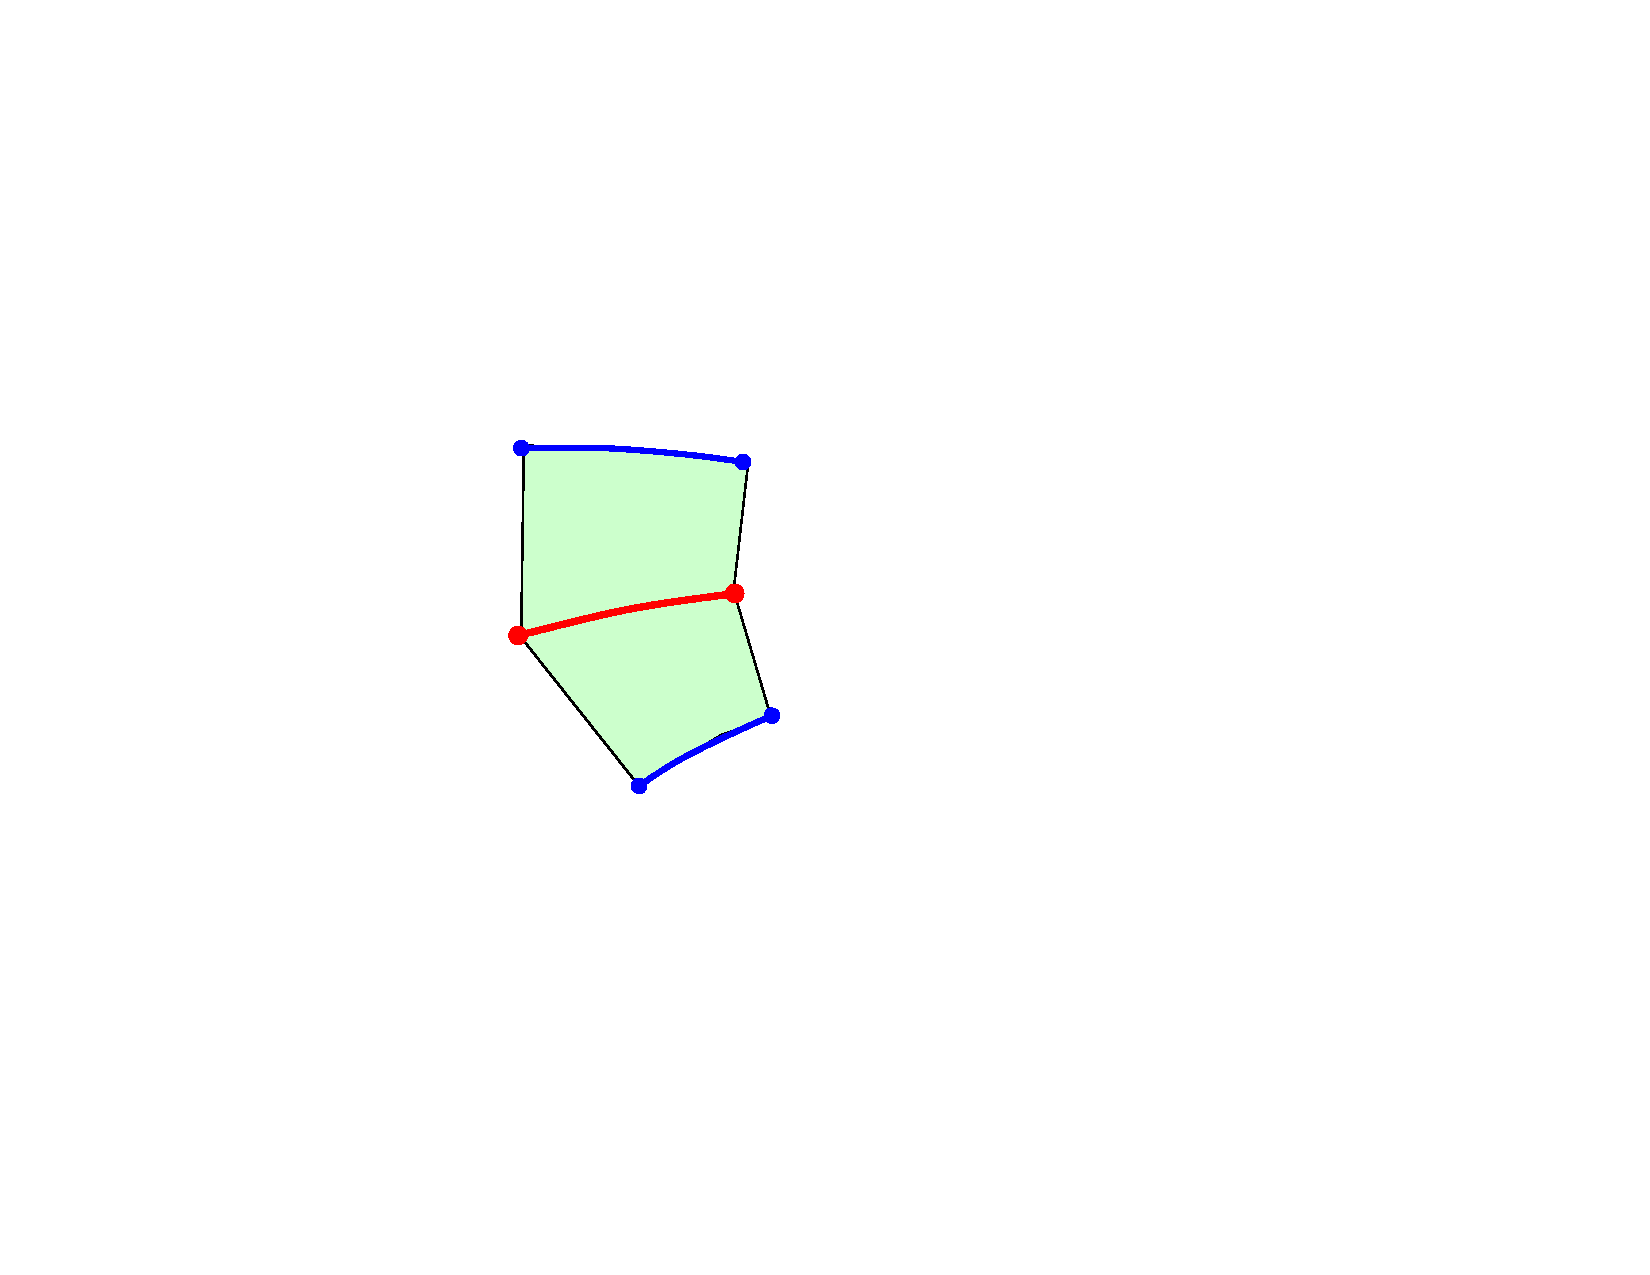
\includegraphics[width=0.2\linewidth]{figs/xshock-fragment-A12.pdf}
b)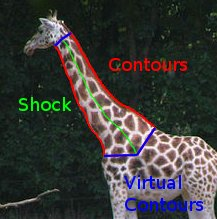
\includegraphics[width=0.25\linewidth]{figs/giraffe-fragment.jpg}
c)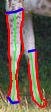
\includegraphics[height=0.25\linewidth]{figs/frontlegs.jpg}
d)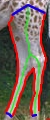
\includegraphics[height=0.25\linewidth]{figs/back_legs.jpg}
%b)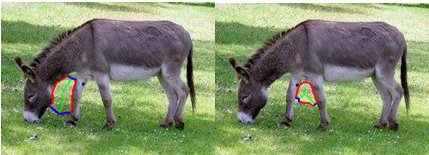
\includegraphics[width=0.45\linewidth]{figs/donkey-fragments-background.jpg}
%d) 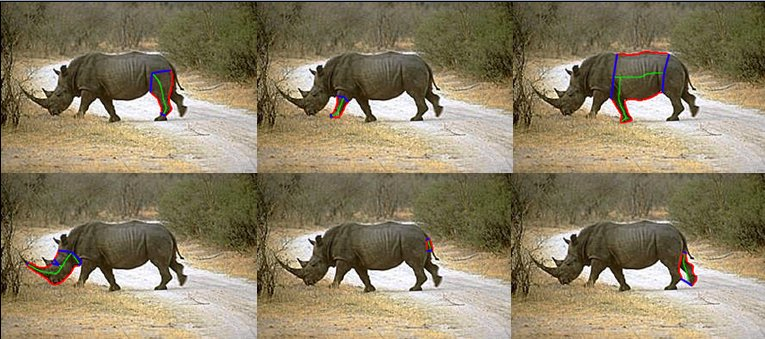
\includegraphics[width=0.48\linewidth]{figs/rhino-fragments-good.jpg}
\caption{ A sketch of a fragment (a), is also sketched on top of an image in (b). Real examples are shown in (c,d) }
  \label{fig:frag_sequence}
 %   %\vspace{-0.3cm}
\end{figure}

\begin{figure*}[ht]
%\vspace{-0.252cm}
\footnotesize{\textit{a}}\hspace{-0.005cm}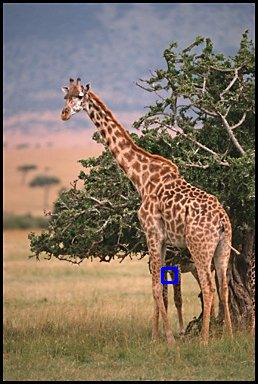
\includegraphics[width=0.24\linewidth]{figs/five_full_image_bbox.jpg}
\footnotesize{\textit{b}}\hspace{-0.005cm}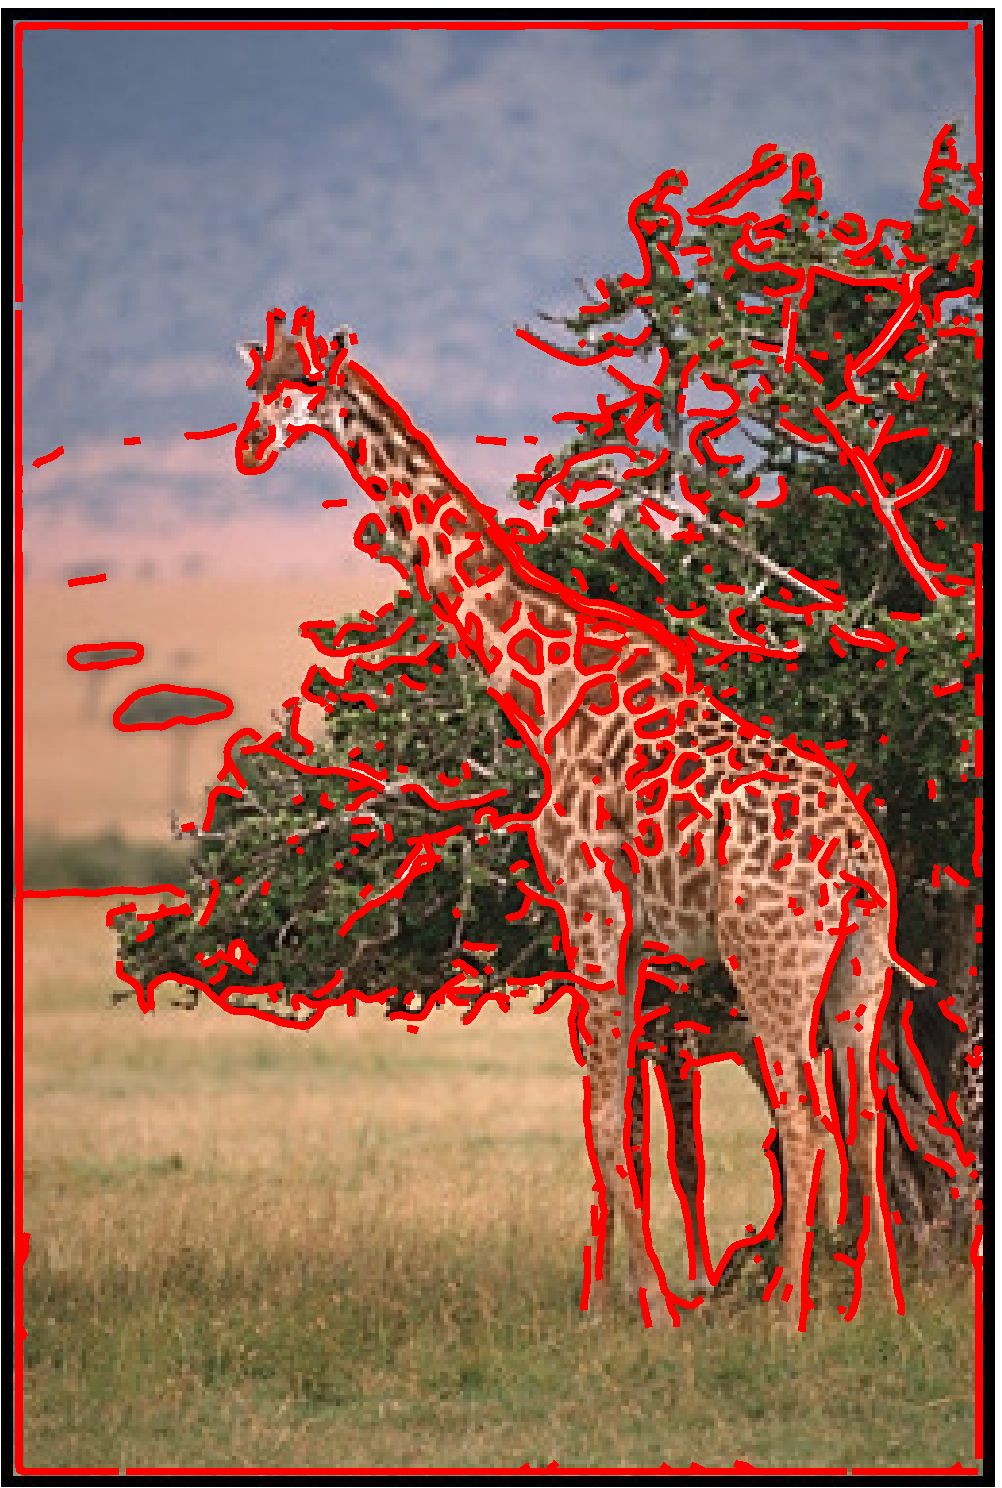
\includegraphics[width=0.24\linewidth]{figs/five_full_image_contours.pdf}
\footnotesize{\textit{c}}\hspace{-0.005cm}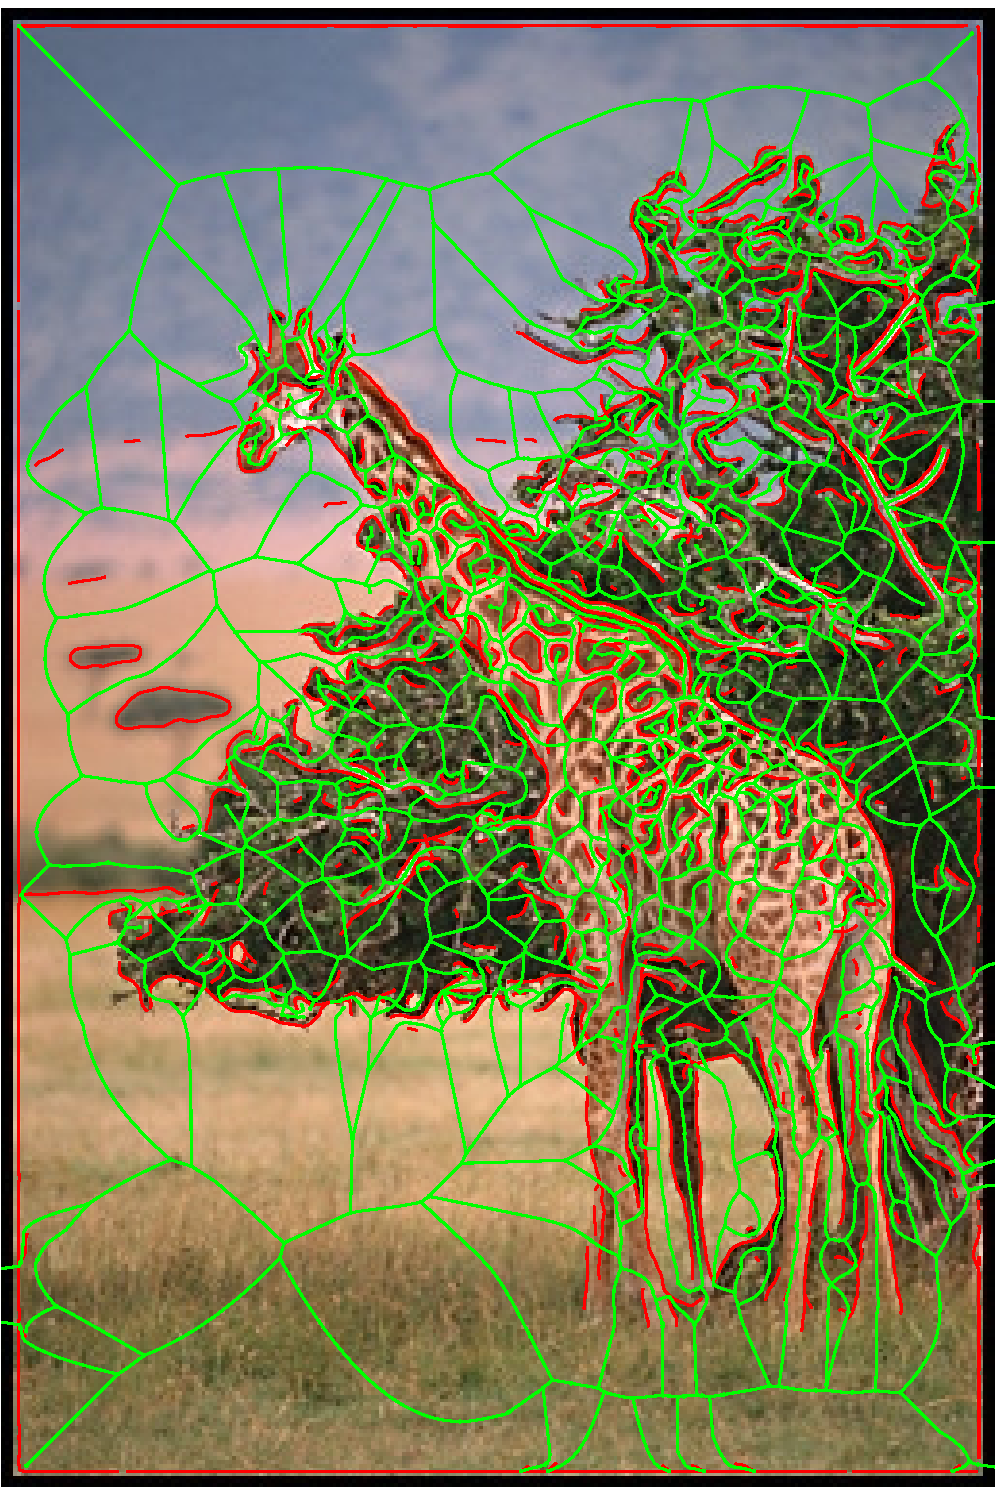
\includegraphics[width=0.24\linewidth]{figs/five_full_image_contours_shocks.pdf}
\footnotesize{\textit{d}}\hspace{-0.005cm}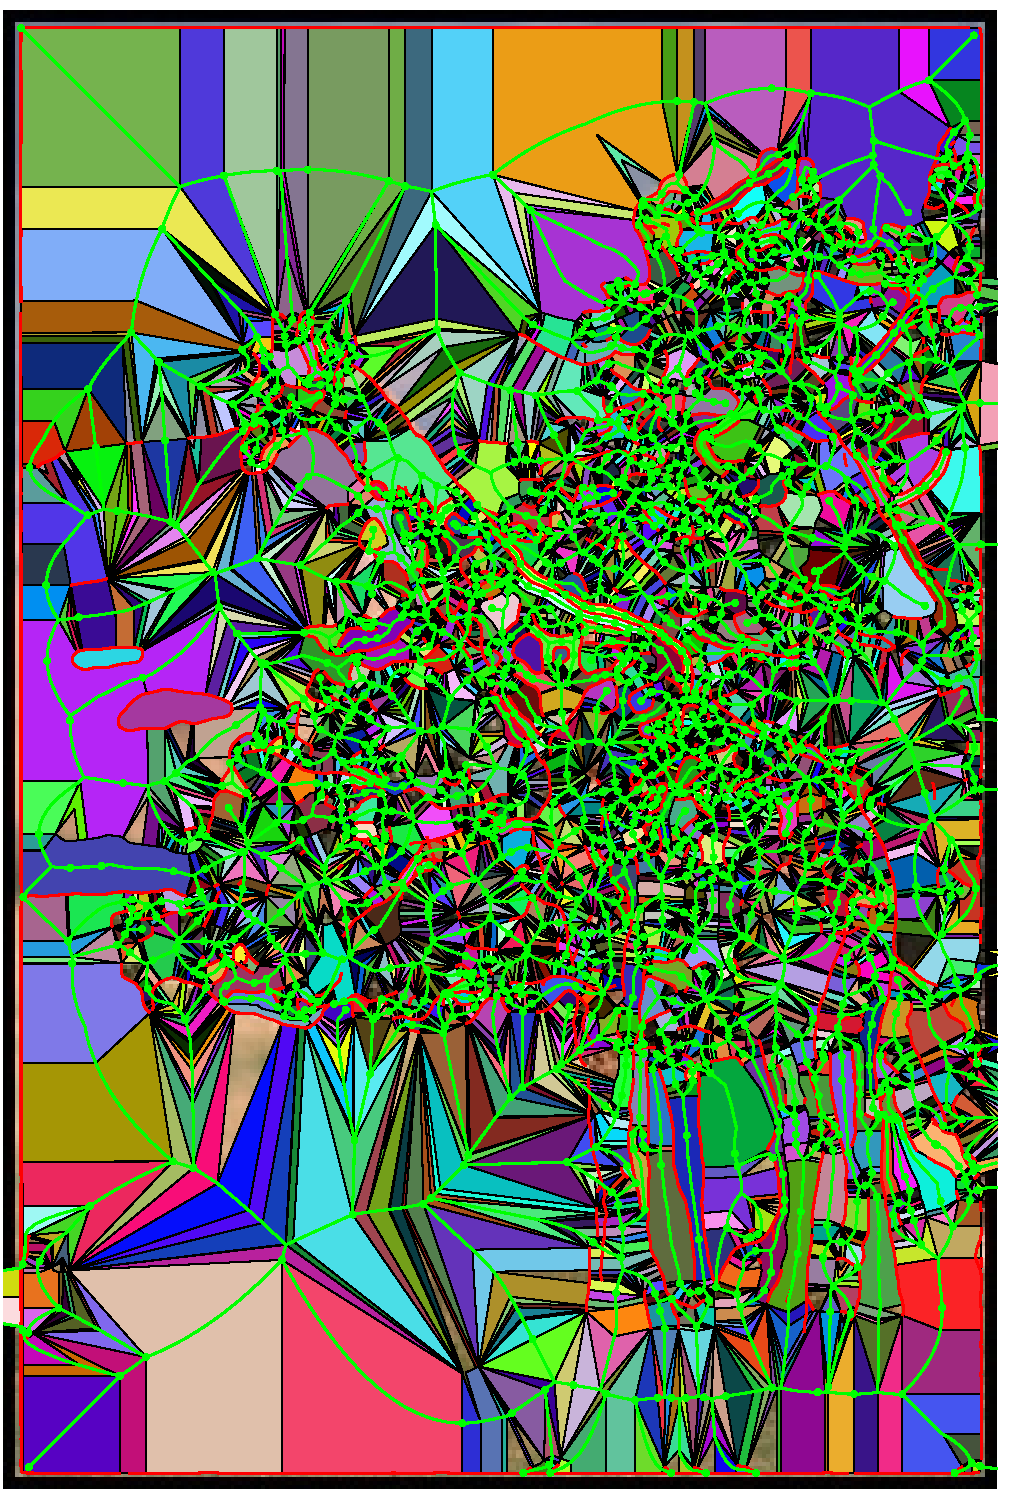
\includegraphics[width=0.24\linewidth]{figs/five_full_image_frags.pdf}\\

\includegraphics[height=0.14\linewidth]{figs/five_local_patch_contours.pdf}
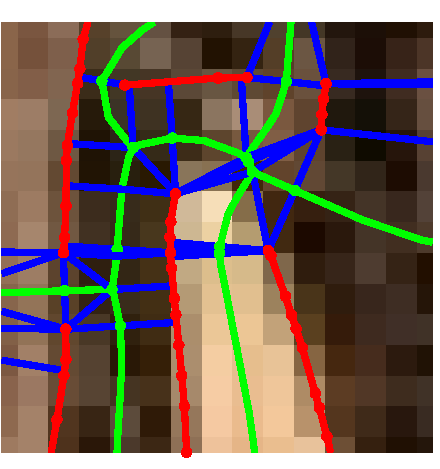
\includegraphics[height=0.14\linewidth]{figs/five_local_patch_contours_shocks.pdf}
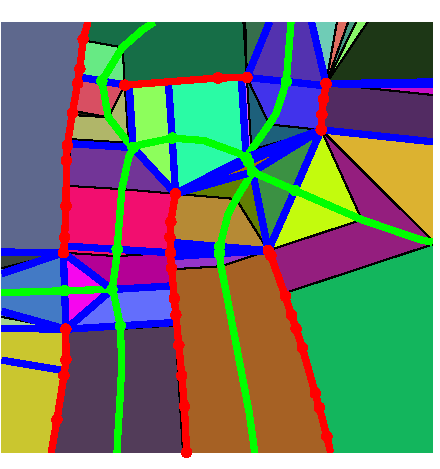
\includegraphics[height=0.14\linewidth]{figs/five_pre_frags_with_contours_shocks.pdf}
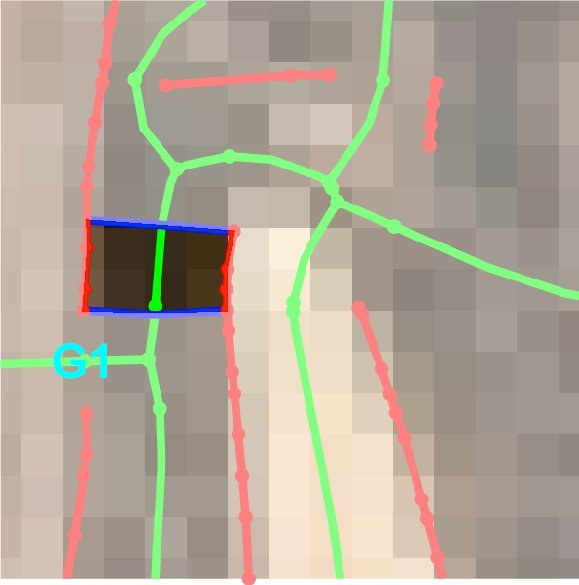
\includegraphics[height=0.14\linewidth]{figs/five_local_patch_highlight_frag.jpg}
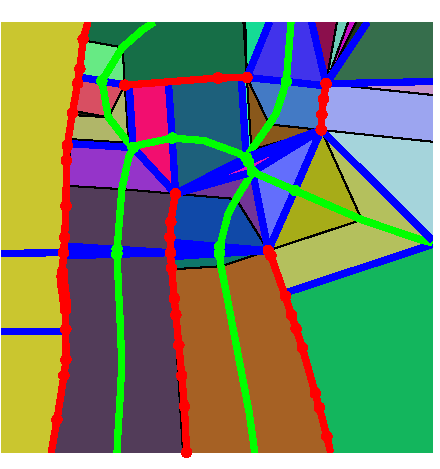
\includegraphics[height=0.14\linewidth]{figs/five_post_frags_with_contours_shocks.pdf}

\includegraphics[height=0.14\linewidth]{figs/five_post_contours.pdf}
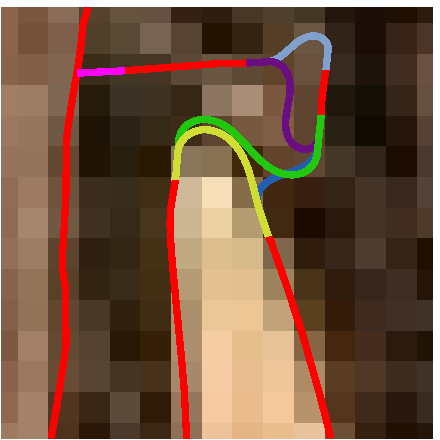
\includegraphics[height=0.14\linewidth]{figs/five_local_patch_gap_hypos.pdf}
\centerline
{
\footnotesize{\textit{(e)}}\hfill
\footnotesize{\textit{(f)}}\hfill
\footnotesize{\textit{(g)}}\hfill
\footnotesize{\textit{(h)}}\hfill
\footnotesize{\textit{(i)}}\hfill
\footnotesize{\textit{(j)}}\hfill
\footnotesize{\textit{(k)}}\hfill
}
%\includegraphics[height=0.135\linewidth]{figs/atomic-fragment.png}
%{\footnotesize\textit{l}} \hspace{-0.0512cm}
%\includegraphics[height=0.135\linewidth]{figs/giraffe-fragment.png}
% {\footnotesize\textit{(m)}}
%\vspace{-0.7cm}
      \caption{\FigureFont (a) The original image, (b) its  contour fragments
in red,
(c) the shock graph in green (the dynamics and types of shocks are not shown,
but are very important), (d) the resulting medial fragments, (e) contour fragments of the
zoomed area in (a), (f)  composite contour and shock graph, (g) 
medial fragments, (h) one medial fragment highlighted, (i) the application of Gap I transform from Figure~\ref{fig:transform:list}; (j) the resulting contours; (k) The next set of potential
completions.}
   \label{fig:frag:definition}
   %\vspace{-0.52cm}
\end{figure*}
  
% 
% \begin{figure}[!h]
%   \centerline{
%     \textit{(a)}  \hspace{-0.2cm}
%     \includegraphics[height=0.253\linewidth]{figs/atomic-fragment.png}
%     % \includegraphics[height=0.253\linewidth]{figs/giraffe-frag-waves.png}
%     \textit{(b)}\includegraphics[height=0.253\linewidth]{figs/giraffe-fragment.png}
%     \textit{(c)}\includegraphics[height=0.253\linewidth]{figs/frag_image_overlay.png}
%   }
%    
% \centerline{\textit{(d)} \includegraphics[height=0.153\linewidth]{figs/tiger-fragments.png}}
% %\includegraphics[height=0.153\linewidth]{figs/tiger_ds.pdf}   
% \caption{\FigureFont (a,b)\ An atomic fragment in the region between two paired boundaries
% and is represented by a shock graph segment. Real contours are in red,
% virtual contours (shock rays) are in blue and shocks are in green. (c)\ Some examples. (d)\   Image, contour
% fragments, the shock graph, and atomic fragments filled in, respectively. }
%    \label{fig:atomic:fragment}
%    %\vspace{-0.5cm}
% \end{figure}
% 
% 
% 
% 



